\documentclass[11pt]{article}

\usepackage{graphicx}

\oddsidemargin0cm
\topmargin-3cm
\textwidth16.0cm
\textheight24.5cm

\newcommand{\step}[2] {\vspace{.25in} \hrule\vspace{0.5em}
  \noindent{\bf Step #1: #2} \vspace{0.5em}
  \hrule \vspace{.10in}}

\begin{document}
\thispagestyle{empty}

\noindent Aaron Gutierrez \& Mitchell Plamann\hfill{15-221}\\
amgutier@andrew.cmu.edu \& mplamann@andrew.cmu.edu \hfill{Spring 2015}\\
Section A \hfill{Team 9}

\vspace{\fill}
\begin{center}
Writing Assignment 3
Instructions

\today
\end{center}
\vspace{\fill}

\newpage

\pagenumbering{arabic}
\begin{center}
{\Huge Creating and Closing GitHub Issues}
\end{center}
\section{Overview}
GitHub provides a great tool for multi-user collaboration on software projects.
On top of the version control features, GitHub offers sophisticated issue
tracking integrated right in with all of your repositories.  Tracking issues
makes it easy to keep track of bugs, new feature ideas, and feedback from
testers, all of which help keep your project organized.  In the next five
steps, you will learn how to create a new issues, assign an issue to a
contributor, and mark an issue as resolved.

This tutorial is for GitHub users who know how to create and use repositories,
but are unfamiliar with GitHub's issue tracking features. You need to have an
existing GitHub repository, a web browser, and a git client on your computer.
Once you're done, you'll be able add, manage, and close issues for every project
you have on GitHub.

\section{Steps}

\step{1}{Open your repository's Issues page}
{\bf In this step, you will access the Issues page for your repository.}

\begin{enumerate}
\item Open your GitHub repository in your web browser.
\item Click ``Issues'' (Fig \ref{fig:issues_button})
\item You should now see the ``Issues'' page, which you will use in Step 2.
\end{enumerate}

\begin{figure}[h]
  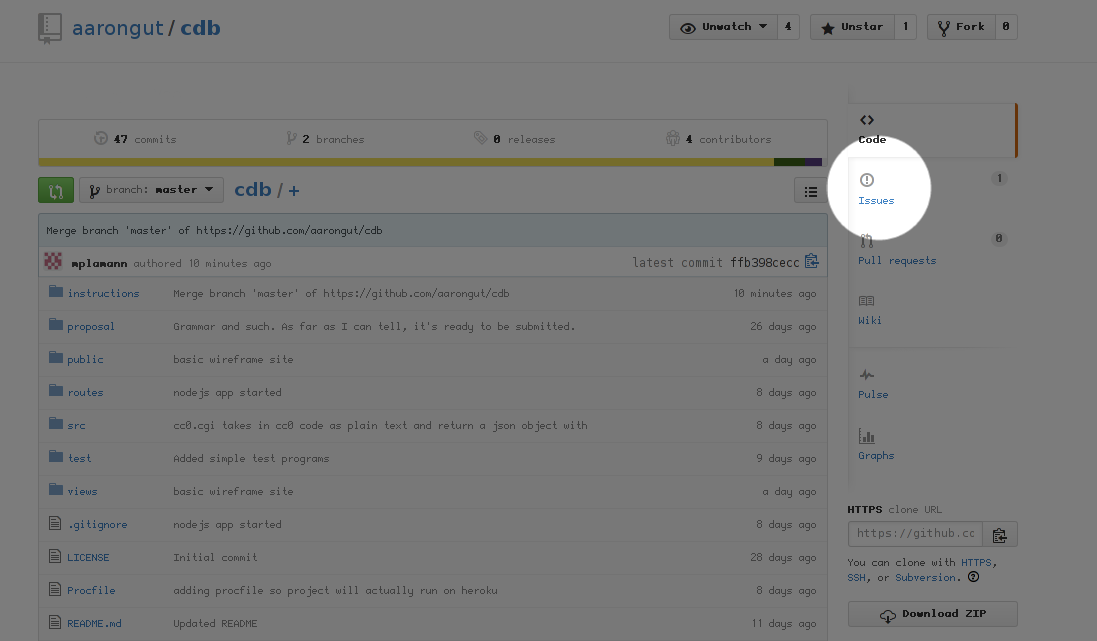
\includegraphics[width=\linewidth]{finding-issues-page-cropped.png}
  \caption{Opening the Issues page}
  \label{fig:issues_button}
\end{figure}

\pagebreak

\step{2}{Create an issue}
{\bf In this step, you will create a new issue associated with your repository and 
fill in necessary information}

\begin{enumerate}
\item Click the ``New Issue'' button (Fig \ref{fig:new_issue})
\item Enter in a title for the issue (1, Fig \ref{fig:issue_info})
\item Enter in a description for the issue (2, Fig \ref{fig:issue_info})
\item Click ``Submit new issue'' (3, Fig \ref{fig:issue_info})
\item Continue to step 3, where you will add a label to your newly-created issue.
\end{enumerate}

\begin{figure}[h]
  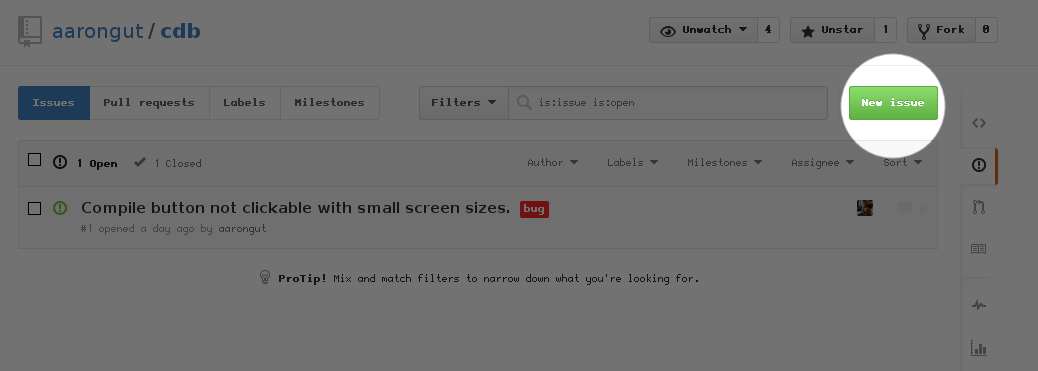
\includegraphics[width=\textwidth]{clickin-new-issue-cropped.png}
  \caption{Creating a new issue}
  \label{fig:new_issue}
\end{figure}

\begin{figure}[h]
  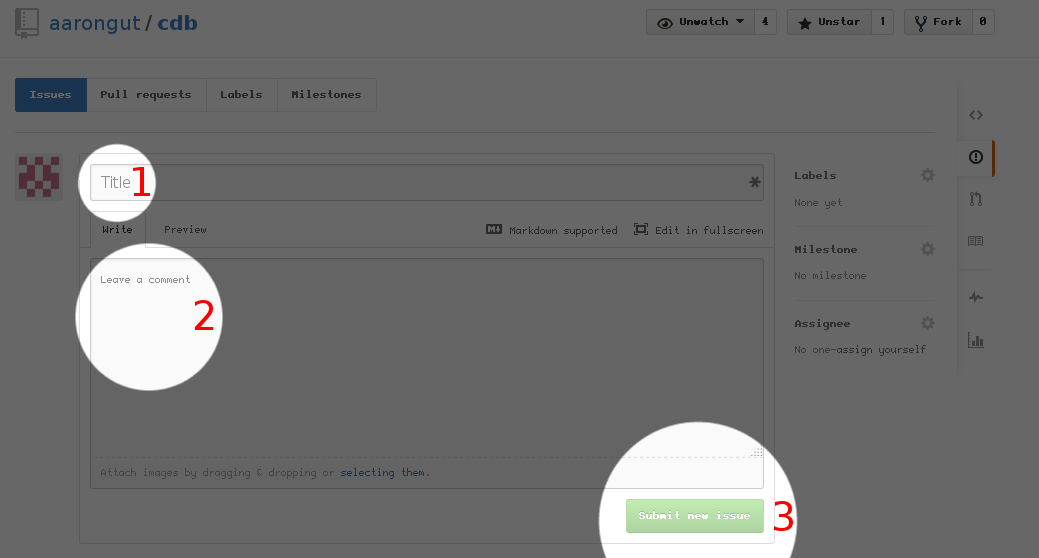
\includegraphics[width=\textwidth]{new-issue-info-cropped.png}
  \caption{Entering issue information}
  \label{fig:issue_info}
\end{figure}

\pagebreak

\step{3}{Assign labels to an issue}
{\bf In this step, you will label your issue, indicating what type of issue it is.}

\begin{enumerate}
\item Click the ``Labels'' button (1, Fig \ref{fig:labels})
\item Click each label that applies to your issue (2, Fig \ref{fig:labels})
\item Click the X button (3, Fig \ref{fig:labels})
\item In step 4, you will assign this issue to a developer.
\end{enumerate}

\begin{figure}[h]
  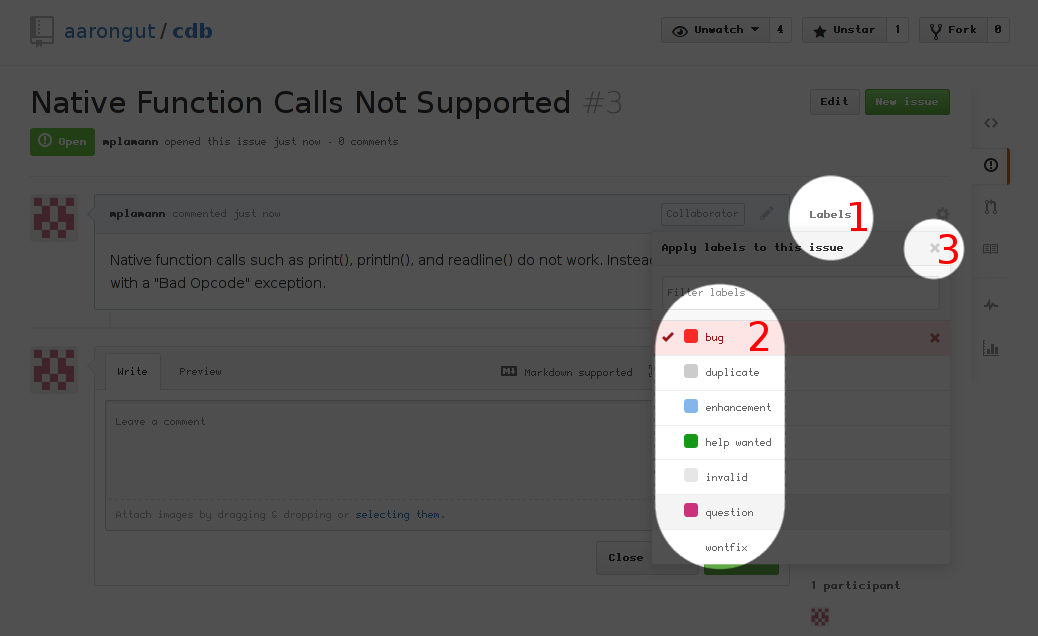
\includegraphics[width=\textwidth]{adding-labels-cropped.png}
  \caption{Adding labels to an issue}
  \label{fig:labels}
\end{figure}

\pagebreak

\step{4}{Assign an issue to a developer}
{\bf In this step, you will assign this issue to a developer who will fix the issue.}

\begin{enumerate}
\item Click the ``Assignee'' button (1, Fig \ref{fig:assign})
\item Click the name of the developer who will fix the issue (2, Fig \ref{fig:assign})
\item At this point, the issue has been assigned to the deveoper.
  Once the developer has fixed the issue, proceed to step 5 to mark the issue as resolved.
\end{enumerate}

\begin{figure}[h]
  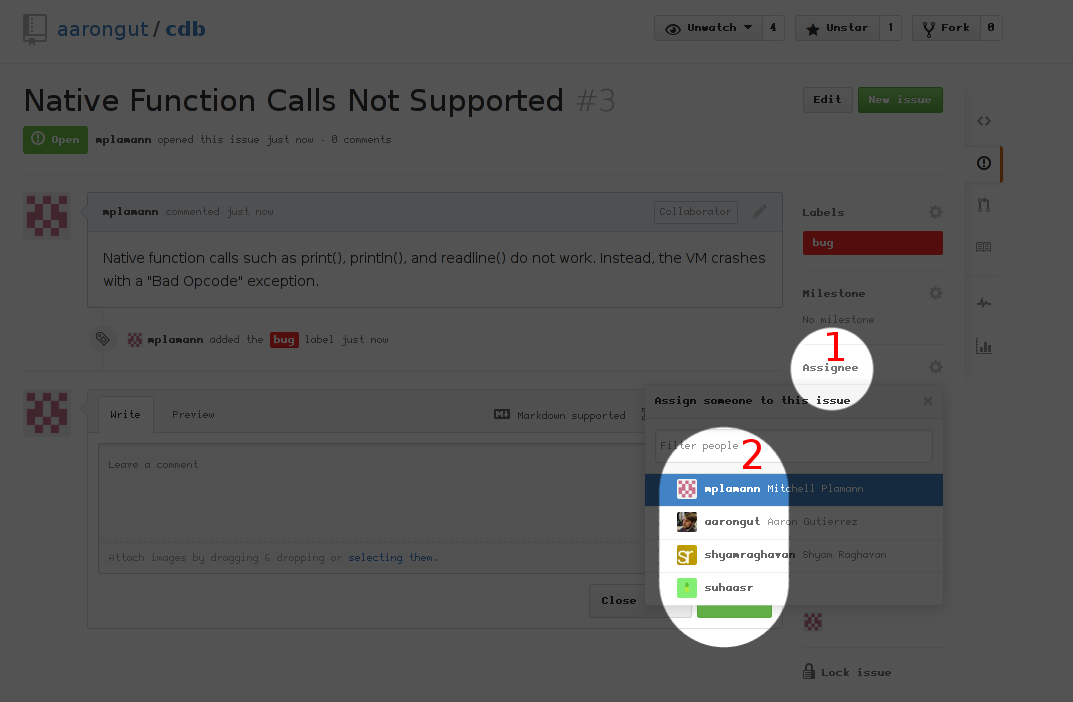
\includegraphics[width=\textwidth]{assign-to-developer-cropped.png}
  \caption{Assigning an issue to a developer}
  \label{fig:assign}
\end{figure}

\pagebreak

\step{5}{Marking an issue as resolved}
{\bf In this step, you will mark the issue as resolved,
  indicating that the developer assigned to the issue has fixed it.}

\begin{enumerate}
\item On the issue web page, you can see the issue number.
  For our example, it is \#3 (Fig \ref{fig:issue_number}).
\item Using your git client on your computer, make a commit as you normally
  would including the changes that fix the issue.  In the commit message,
  include the text ``Resolves \#{\it N}'', replacing {\it N} with your issue number.  In
  the example issue, the commit message would be ``Resolves \#3''.
\item GitHub detects this commit and marks the issue as closed (Fig \ref{fig:resolved}).
  At this point, you have successfully created a GitHub issue, fixed the problem in the repository,
  and marked the issue as resolved.
\end{enumerate}

\begin{figure}[h]
  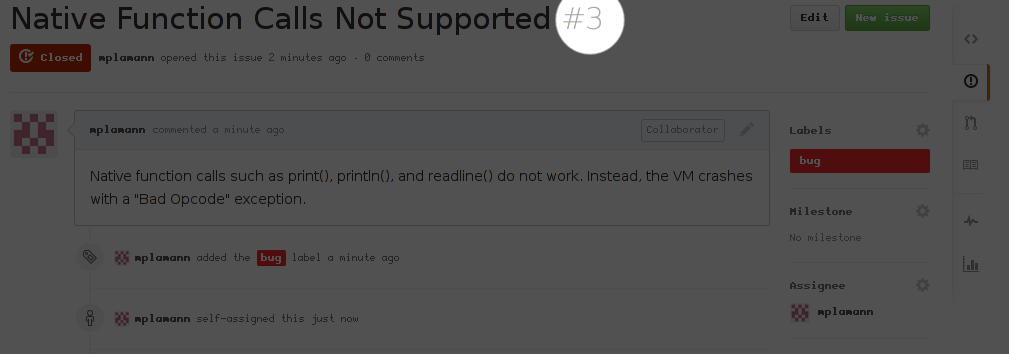
\includegraphics[width=\textwidth]{issue-number-cropped.png}
  \caption{Finding the issue number}
  \label{fig:issue_number}
\end{figure}

\begin{figure}[h]
  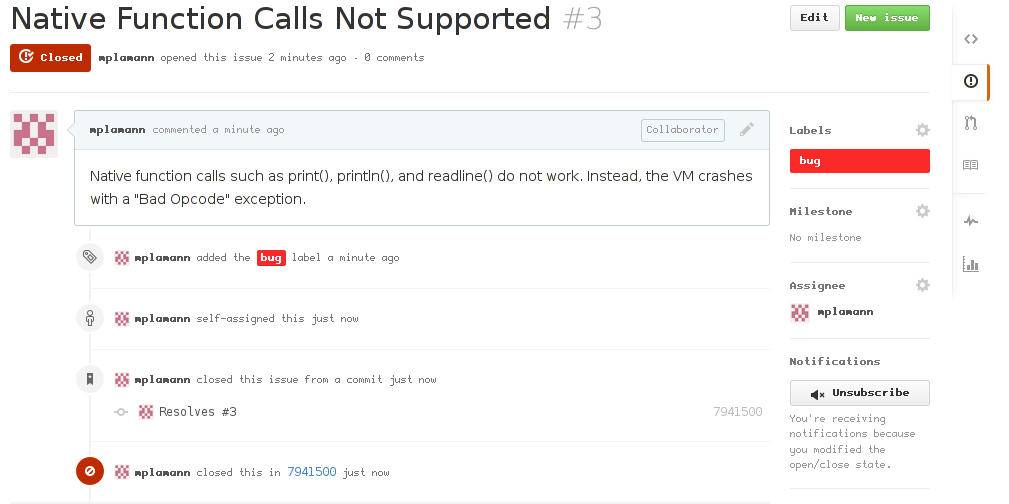
\includegraphics[width=\textwidth]{issue-resolved-cropped.png}
  \caption{The issue has been resolved}
  \label{fig:resolved}
\end{figure}

\end{document}
